\chapter{Bioinformática y análisis de secuencias}\label{ch:b3:bioinformatics}

Un biólogo que acaba de secuenciar un gen de un gusano abisal pega sus
\num{300} aminoácidos en un formulario web y, tres segundos después,
descubre que la proteína es prima lejana de una quinasa humana, con un
\qty{31}{\%} de identidad a lo largo de \num{280} residuos y una
probabilidad de $10^{-40}$ de que el parecido sea azar. Detrás de esos
tres segundos hay un algoritmo de \omterm{thm:b3:bioinformatics:nw}{programación dinámica} de 1970, una
teoría estadística de los \omterm{def:b3:bioinformatics:alignment}{alineamientos} aleatorios, matrices de
sustitución destiladas de miles de familias de proteínas y una base de
datos de unos cien mil millones de residuos. Este capítulo trata del
razonamiento que hay dentro de la caja: cómo se alinean dos secuencias de
manera que el \omterm{def:b3:bioinformatics:alignment}{alineamiento} sea demostrablemente el mejor, cómo se logra
que la puntuación signifique algo, cómo se distingue una coincidencia de
una casualidad y cómo se encuentran patrones en un genoma que nadie ha
mirado antes. La matemática es elemental --- una recurrencia, un
logaritmo, una distribución de Poisson --- y conviene conocerla, porque
toda conclusión extraída de una comparación de secuencias descansa en ella.

\section{Alinear dos secuencias}

\begin{definition}[Alineamiento y puntuación]\label{def:b3:bioinformatics:alignment}
\index{alineamiento de secuencias}\index{penalización por hueco}\index{alineamiento global}\index{alineamiento local}
Un \emph{alineamiento} de dos secuencias las escribe una sobre la otra,
con \emph{huecos} (--) insertados de modo que las columnas emparejen un
residuo con un residuo o un residuo con un hueco, y ninguna columna
empareje dos huecos. Su \emph{puntuación} es la suma, sobre las columnas,
de una puntuación de sustitución $s(a,b)$ por cada par de residuos y de
una \emph{penalización por hueco} por cada hueco: una penalización lineal
$-d$ por posición de hueco o, de forma más realista, una penalización
\emph{afín} $-d - (k-1)e$ por una tirada de $k$ huecos, con un coste de
apertura $d$ mayor que el coste de extensión $e$, ya que una sola
inserción de varios residuos es un único suceso evolutivo. Un
alineamiento \emph{global} cubre ambas secuencias de extremo a extremo;
un alineamiento \emph{local} halla el par de subcadenas de mayor
puntuación e ignora el resto, que es lo que uno quiere cuando un dominio
compartido se sitúa en dos proteínas por lo demás no emparentadas.
\end{definition}

\begin{theorem}[Needleman--Wunsch]\label{thm:b3:bioinformatics:nw}
\index{Needleman--Wunsch}\index{programación dinámica}\index{Smith--Waterman}
Sean $x = x_{1}\dots x_{m}$ e $y = y_{1}\dots y_{n}$, con penalización
lineal por hueco $d$. Defínase $F(i,j)$ como la mejor puntuación de un
\omterm{def:b3:bioinformatics:alignment}{alineamiento global} de los prefijos $x_{1}\dots x_{i}$ e
$y_{1}\dots y_{j}$. Entonces $F(i,0) = -id$, $F(0,j) = -jd$ y, para
$i,j \ge 1$,
\[
F(i,j) = \max\bigl\{\,F(i-1,j-1) + s(x_{i},y_{j}),\;
F(i-1,j) - d,\; F(i,j-1) - d\,\bigr\}.
\]
$F(m,n)$ es la puntuación global óptima, un \omterm{def:b3:bioinformatics:alignment}{alineamiento} óptimo se
recupera siguiendo hacia atrás desde $(m,n)$ las decisiones que
produjeron cada máximo, y todo el cálculo cuesta $mn$ pasos. La variante
de \emph{Smith--Waterman} para el \omterm{def:b3:bioinformatics:alignment}{alineamiento local} añade $0$ como
cuarta opción del máximo, pone los bordes a $0$ y lee la respuesta en la
mayor entrada de la tabla.
\end{theorem}
\begin{proof}
Considérese la última columna de cualquier \omterm{def:b3:bioinformatics:alignment}{alineamiento} de los dos
prefijos. Es una de tres cosas: $x_{i}$ sobre $y_{j}$, $x_{i}$ sobre un
hueco o un hueco sobre $y_{j}$. Quitarla deja un \omterm{def:b3:bioinformatics:alignment}{alineamiento} de
$(x_{1}\dots x_{i-1},
y_{1}\dots y_{j-1})$, de $(x_{1}\dots x_{i-1}, y_{1}\dots y_{j})$ o de
$(x_{1}\dots x_{i}, y_{1}\dots y_{j-1})$ respectivamente, cuya puntuación
es como mucho $F$ de ese par; y, a la inversa, cada uno de esos
\omterm{def:b3:bioinformatics:alignment}{alineamientos} óptimos puede extenderse con la última columna
correspondiente. Así que la mejor puntuación que termina en cada tipo de
columna es $F$ del par más corto más la puntuación de la columna, y el
óptimo es el mayor de los tres. Los bordes están forzados (contra un
prefijo vacío solo caben huecos). La inducción sobre $i + j$ rellena la
tabla; el número de celdas es $(m+1)(n+1)$. Para el \omterm{def:b3:bioinformatics:alignment}{alineamiento local} la
opción adicional $0$ significa ``empiécese aquí un \omterm{def:b3:bioinformatics:alignment}{alineamiento} nuevo'',
lo que hace de $F(i,j)$ la mejor puntuación de un \omterm{def:b3:bioinformatics:alignment}{alineamiento} que
\emph{termina} en $(i,j)$, y el mejor \omterm{def:b3:bioinformatics:alignment}{alineamiento local} termina en algún
sitio.
\end{proof}

\begin{example}[Una tabla de cuatro por tres]\label{ex:b3:bioinformatics:nw-example}
Alinéese GAT con GCAT, puntuando $+1$ una coincidencia, $-1$ una
discrepancia y $d = 1$. Los bordes son $0, -1, -2, -3, -4$ a lo largo de
la fila superior y $0, -1,
-2, -3$ por el lado. Rellenando fila a fila: $F(\text{G},\text{G}) = 1$,
$F(\text{G},\text{C}) = 0$, $F(\text{G},\text{A}) = -1$,
$F(\text{G},\text{T}) = -2$; $F(\text{A},\text{G}) = 0$,
$F(\text{A},\text{C}) = 0$, $F(\text{A},\text{A}) = 1$,
$F(\text{A},\text{T}) = 0$; $F(\text{T},\text{G}) = -1$,
$F(\text{T},\text{C}) = -1$, $F(\text{T},\text{A}) = 0$,
$F(\text{T},\text{T}) = 2$. El óptimo es $2$, y siguiendo hacia atrás
--- diagonal desde (T,T), diagonal desde (A,A), luego a la izquierda de
(G,C) a (G,G) y después diagonal --- se obtiene
\[
\begin{array}{c}
\texttt{G-AT}\\
\texttt{GCAT}
\end{array}
\]
tres coincidencias y un hueco: $3 - 1 = 2$.
\end{example}

\begin{omfigure}
\begin{tikzpicture}[every node/.style={font=\small}, >=stealth]
  \def\dx{1.0}\def\dy{0.8}
  % headers
  \foreach \j/\c in {1/G,2/C,3/A,4/T} \node[omDef, font=\small\bfseries] at (\j*\dx+0.5,0.4) {\c};
  \foreach \i/\c in {1/G,2/A,3/T} \node[omDef, font=\small\bfseries] at (-0.5,-\i*\dy-0.4) {\c};
  % grid
  \draw[gray!60] (0,0) grid[xstep=\dx, ystep=\dy] (5*\dx,-4*\dy);
  % values
  \foreach \i/\j/\v in {0/0/0,0/1/-1,0/2/-2,0/3/-3,0/4/-4,1/0/-1,2/0/-2,3/0/-3, 1/1/1,1/2/0,1/3/-1,1/4/-2, 2/1/0,2/2/0,2/3/1,2/4/0, 3/1/-1,3/2/-1,3/3/0,3/4/2}
    \node at (\j*\dx+0.5,-\i*\dy-0.4) {$\v$};
  % traceback path highlighted
  \foreach \i/\j in {0/0,1/1,1/2,2/3,3/4} \draw[omThm, very thick] (\j*\dx+0.05,-\i*\dy-0.05) rectangle (\j*\dx+\dx-0.05,-\i*\dy-\dy+0.05);
  \draw[->, omThm, very thick, shorten >=8pt, shorten <=8pt] (4.5,-2.8) -- (3.5,-2.0);
  \draw[->, omThm, very thick, shorten >=8pt, shorten <=8pt] (3.5,-2.0) -- (2.5,-1.2);
  \draw[->, omThm, very thick, shorten >=8pt, shorten <=8pt] (2.5,-1.2) -- (1.5,-1.2);
  \draw[->, omThm, very thick, shorten >=8pt, shorten <=8pt] (1.5,-1.2) -- (0.5,-0.4);
  \node[right, align=left] at (5.6,-1.6) {traza atrás desde $F(3,4) = 2$:\\diagonal, diagonal,\\izquierda (hueco en GAT), diagonal\\[3pt] \texttt{G-AT}\\\texttt{GCAT}};
\end{tikzpicture}

{\small La tabla de Needleman--Wunsch para GAT contra GCAT (coincidencia
$+1$, discrepancia $-1$, hueco $-1$). Cada celda es la mejor puntuación
de los dos prefijos que terminan ahí; el camino rojo trazado hacia atrás
desde la esquina es el \omterm{def:b3:bioinformatics:alignment}{alineamiento} óptimo.}
\end{omfigure}

\begin{method}[Alinear dos secuencias]\label{met:b3:bioinformatics:align}
\index{traza atrás}
(1) Elíjase la puntuación: una \omterm{def:b3:bioinformatics:matrices}{matriz de sustitución} adecuada a la
divergencia esperada (BLOSUM62 para proteínas de distancia desconocida;
coincidencia y discrepancia para el ADN) y penalizaciones afines por
hueco (típicamente apertura $-11$ y extensión $-1$ con BLOSUM62).
(2) Decídase global o local: global para dos secuencias que se creen
homólogas en toda su longitud, y local en los demás casos. (3) Rellénese
la tabla con la recurrencia, guardando en cada celda un puntero a la
decisión que dio su máximo. (4) Trácese hacia atrás desde $(m,n)$ (en el
global) o desde la celda máxima hasta un cero (en el local), escribiendo
el \omterm{def:b3:bioinformatics:alignment}{alineamiento} de derecha a izquierda. (5) Júzguese el resultado no por
su puntuación bruta sino por su significación estadística (más abajo), y
mírese: los huecos largos, las tiradas de baja complejidad y los
\omterm{def:b3:bioinformatics:alignment}{alineamientos} confinados a una repetición son avisos.
\end{method}

\section{Puntuar: cuánto vale una coincidencia}

\begin{definition}[Matrices de sustitución]\label{def:b3:bioinformatics:matrices}
\index{matriz de sustitución}\index{BLOSUM}\index{PAM}\index{puntuación de log-verosimilitudes}
Una \emph{matriz de sustitución} da $s(a,b)$ para cada par de
aminoácidos como una \emph{puntuación de log-verosimilitudes}:
\[
s(a,b) = \frac{1}{\lambda}\,\log\frac{q_{ab}}{p_{a}\,p_{b}},
\]
donde $q_{ab}$ es la frecuencia con la que $a$ y $b$ aparecen alineados
en \omterm{def:b3:bioinformatics:alignment}{alineamientos} fiables de proteínas emparentadas, $p_{a} p_{b}$ la
frecuencia con la que se emparejarían por azar y $\lambda$ una escala
elegida para que las entradas sean enteros cómodos. Una puntuación
positiva significa que el par aparece más a menudo en homólogos que por
azar; las puntuaciones de identidad son mayores para los aminoácidos
raros (triptófano $+11$, cisteína $+9$ en BLOSUM62) y menores para los
frecuentes (leucina $+4$, alanina $+4$), y las sustituciones
conservadoras (isoleucina--valina $+3$) puntúan positivo mientras que las
radicales (triptófano--glicina $-2$) puntúan negativo. Las matrices
\emph{PAM} (Dayhoff, 1978) se dedujeron de proteínas muy próximas y se
extrapolaron a distancias mayores por multiplicación de matrices; las
matrices \emph{BLOSUM} (Henikoff y Henikoff, 1992) se contaron
directamente en bloques de secuencias alineadas agrupadas a una identidad
dada --- BLOSUM62 a partir de bloques al \qty{62}{\%} --- y son las
predeterminadas porque se midieron, en lugar de extrapolarse, a la
distancia a la que se usan.
\end{definition}

\begin{proposition}[Por qué log-verosimilitudes]\label{prop:b3:bioinformatics:logodds}
\index{puntuación esperada}
Para que un esquema de puntuación pueda usarse en \omterm{def:b3:bioinformatics:alignment}{alineamiento local}, la
\omterm{prop:b3:bioinformatics:logodds}{puntuación esperada} de una columna emparejada al azar,
$\sum_{a,b} p_{a} p_{b}\, s(a,b)$, ha de ser negativa, y algunas
puntuaciones han de ser positivas; de lo contrario los \omterm{def:b3:bioinformatics:alignment}{alineamientos}
aleatorios crecerían sin límite y el segmento de mayor puntuación sería
la secuencia entera. Dado eso, todo esquema de esa clase es equivalente a
un esquema de log-verosimilitudes para \emph{algunas} frecuencias
objetivo $q_{ab}$ --- los \omterm{def:b3:bioinformatics:alignment}{alineamientos} que encontrará como óptimos son
aquellos cuyos pares de residuos se distribuyen como $q_{ab}$. Elegir la
matriz es por tanto elegir la divergencia que se espera detectar: una
matriz para parientes próximos (BLOSUM80, PAM30) tiene positivos más
marcados y negativos más duros, y una para parientes lejanos (BLOSUM45,
PAM250) es más plana.
\end{proposition}
\admitted

\begin{example}[Identidad, similitud y la zona crepuscular]\label{ex:b3:bioinformatics:twilight}
Dos secuencias de proteína aleatorias alineadas de forma óptima con
huecos alcanzan por azar entre el \qtyrange{15}{20}{\%} de identidad. Por
encima del \qty{35}{\%} de identidad a lo largo de cien residuos, dos
proteínas son casi con seguridad homólogas; entre el \qty{20}{\%} y el
\qty{35}{\%} está la \emph{zona crepuscular}, donde la identidad por sí
sola no decide y debe hacerlo la estadística de más abajo. Los homólogos
pueden caer muy por debajo de la zona: las subunidades de la hemoglobina
y la mioglobina comparten un \qty{25}{\%} de identidad, la lisozima y la
$\alpha$-lactalbúmina un \qty{40}{\%}, y muchos pares de proteínas con el
mismo plegamiento comparten menos del \qty{15}{\%}, detectable solo
comparando \omterm{def:b3:bioinformatics:msa}{perfiles} o estructuras.
\end{example}

\section{Buscar en una base de datos}

\begin{definition}[BLAST]\label{def:b3:bioinformatics:blast}
\index{BLAST}\index{semilla}\index{par de segmentos de alta puntuación}
Alinear una consulta de \num{300} residuos contra una base de datos de
$10^{11}$ por \omterm{thm:b3:bioinformatics:nw}{programación dinámica} completa costaría $3\times 10^{13}$
actualizaciones de celda por búsqueda. \emph{BLAST} (Altschul y
colaboradores, 1990) cambia un poco de sensibilidad por mil veces más
velocidad en tres pasos: (1) se listan las \emph{palabras} de la consulta
(tres residuos para proteínas, once bases para ADN) y sus vecinas de alta
puntuación; (2) se rastrea la base de datos en busca de coincidencias
exactas de palabra --- las \emph{semillas}; (3) se extiende cada semilla
en ambas direcciones sin huecos hasta que la puntuación cae una cantidad
fijada por debajo de su máximo, conservando los \emph{pares de segmentos
de alta puntuación} (HSP), y luego se unen los HSP próximos con
\omterm{thm:b3:bioinformatics:nw}{programación dinámica} con huecos en una banda estrecha. Un homólogo
verdadero contiene casi siempre al menos una palabra exacta de tres
residuos en común; un parecido casual rara vez la tiene, y nunca se
extiende.
\end{definition}

\begin{omfigure}
\begin{tikzpicture}[every node/.style={font=\scriptsize}, >=stealth]
  % query and database sequences as bars
  \draw[very thick, omDef] (0,2.0) -- (5,2.0); \node[left] at (-0.1,2.0) {consulta};
  \draw[very thick, gray] (0,0.6) -- (11,0.6); \node[left] at (-0.1,0.6) {base de datos};
  % seeds
  \foreach \q/\d in {1.2/3.6, 2.8/5.2, 4.1/9.3} {
    \fill[omThm] (\q-0.15,1.9) rectangle (\q+0.15,2.1);
    \fill[omThm] (\d-0.15,0.5) rectangle (\d+0.15,0.7);
    \draw[omThm, thick] (\q,1.85) -- (\d,0.75);
  }
  \node[above] at (1.2,2.15) {palabra}; \node[above] at (2.8,2.15) {palabra}; \node[above] at (4.1,2.15) {palabra};
  % extension of the first two (same diagonal) -> HSP
  \draw[<->, very thick, omMeth!70!black] (2.6,0.3) -- (6.2,0.3); \node[below] at (4.4,0.25) {extensión sin huecos: un HSP};
  % third seed: extension fails
  \draw[omProp, thick, dashed] (8.8,0.3) -- (9.8,0.3); \node[below, omProp] at (9.3,0.25) {la puntuación cae: descartada};
  \node[right, align=left] at (5.5,2.0) {1. palabras de la consulta\\2. aciertos exactos en la base (semillas)\\3. extensión y conservación de los pares altos};
\end{tikzpicture}

{\small La heurística de \omterm{def:b3:bioinformatics:blast}{BLAST}. Las palabras exactas cortas compartidas
por la consulta y la entrada de la base de datos (rojo) son \omterm{def:b3:bioinformatics:blast}{semillas};
cada una se extiende a lo largo de su diagonal mientras la puntuación
sigue subiendo, y solo las extensiones que se mantienen altas llegan a
ser \omterm{def:b3:bioinformatics:blast}{pares de segmentos de alta puntuación}.}
\end{omfigure}

\begin{theorem}[La estadística de un acierto por azar]\label{thm:b3:bioinformatics:evalue}
\index{valor E}\index{puntuación en bits}\index{Karlin--Altschul}
Para una consulta de longitud $m$ buscada en una base de datos de
longitud total $n$, con un esquema de puntuación de esperanza negativa,
el número de \omterm{def:b3:bioinformatics:alignment}{alineamientos locales} sin huecos que puntúan al menos $S$ y
que surgen por azar sigue una Poisson de media
\[
E = K\,m\,n\,e^{-\lambda S},
\]
donde $\lambda$ y $K$ solo dependen del esquema de puntuación y de las
frecuencias de residuos ($\lambda$ es la escala de la matriz de
log-verosimilitudes). $E$ es el \emph{valor esperado} de la puntuación
$S$. Escribiendo la puntuación en \emph{bits},
$S' = (\lambda S - \ln K)/\ln 2$, la fórmula queda $E = m n\, 2^{-S'}$,
y la probabilidad de que
al menos un \omterm{def:b3:bioinformatics:alignment}{alineamiento} por azar alcance $S$ es $P = 1 - e^{-E}$, que
vale $E$ cuando $E$ es pequeño.
\end{theorem}
\begin{proof}[Demostración parcial]
La cola exponencial es el teorema de Karlin--Altschul y se admite: la
puntuación máxima de un segmento en un paseo aleatorio con deriva
negativa tiene una distribución cuya cola decae como $e^{-\lambda S}$,
con $\lambda$ la raíz positiva de
$\sum_{a,b} p_{a} p_{b} e^{\lambda s(a,b)} = 1$ --- que es exactamente la
ecuación que hace coherente la matriz de log-verosimilitudes. Dada esa
cola, el resto es contar. Los segmentos de alta puntuación pueden empezar
en cualquiera de los $mn$ pares de posiciones, son raros y son casi
independientes; el número de los que superan $S$ sigue por tanto una
Poisson de media proporcional a $mn$ y a la probabilidad de la cola,
$E = Kmn\,e^{-\lambda S}$. La probabilidad de que no haya ninguno es
$e^{-E}$. La sustitución por la \omterm{thm:b3:bioinformatics:evalue}{puntuación en bits} es álgebra:
$e^{-\lambda S} K = 2^{-(\lambda S -
\ln K)/\ln 2}$. Para los \omterm{def:b3:bioinformatics:alignment}{alineamientos} con huecos vale la misma forma con
$\lambda$ y $K$ estimados por simulación.
\end{proof}

\begin{example}[Leer un valor E]\label{ex:b3:bioinformatics:evalue}
Una consulta de \num{250} residuos contra una base de datos de
$5\times 10^{10}$ residuos tiene
$mn = 1.25\times 10^{13} \approx 2^{43.5}$. Un acierto con una
\omterm{thm:b3:bioinformatics:evalue}{puntuación en bits} de $60$ tiene
$E = 2^{43.5 - 60} = 2^{-16.5} \approx 10^{-5}$: es homólogo con
certeza prácticamente absoluta. Un acierto con $S' = 40$ tiene $E = 2^{3.5}
\approx 11$: se esperan once puntuaciones así por azar, y el acierto no
significa nada. El \emph{mismo} \omterm{def:b3:bioinformatics:alignment}{alineamiento}, con la misma \omterm{thm:b3:bioinformatics:evalue}{puntuación en
bits}, buscado en una base de datos diez veces mayor, tiene un $E$ diez
veces mayor --- la significación es una propiedad de la búsqueda, no del
par. El umbral de uso común es $E < 10^{-3}$ para un homólogo fiable;
$E \approx 0.01$--$1$ merece una segunda mirada con un método de \omterm{def:b3:bioinformatics:msa}{perfil}.
\end{example}

\begin{omfigure}
\begin{tikzpicture}
\begin{axis}[
  width=0.7\linewidth, height=5.6cm,
  axis x line=bottom, axis y line=left,
  xmin=25, xmax=70, ymin=0.000000001, ymax=100000000, ymode=log,
  xlabel={puntuación en bits $S'$}, ylabel={$E$},
  xlabel style={font=\small, at={(axis description cs:0.5,-0.12)}, anchor=north},
  ylabel style={font=\small},
  tick label style={font=\small}, xtick={30,40,50,60,70},
  clip=false,
]
\addplot[very thick, omDef, domain=25:70, samples=2] {2^(43.5-x)};
\addplot[very thick, omThm, domain=25:70, samples=2] {2^(46.8-x)};
\addplot[dashed, gray, domain=25:70, samples=2] {0.001};
\node[font=\scriptsize, gray, anchor=south west] at (axis cs:25.5,0.0012) {$E = 10^{-3}$};
\node[font=\scriptsize, omDef, anchor=north west] at (axis cs:26,0.00002) {$mn = 1.25\times 10^{13}$};
\node[font=\scriptsize, omThm, anchor=south west] at (axis cs:45,30) {$mn$ diez veces mayor};
\end{axis}
\end{tikzpicture}

{\small $E = mn\,2^{-S'}$: cada bit adicional reduce a la mitad el número
esperado de aciertos por azar, y una base de datos diez veces mayor
cuesta $3.3$ bits de significación para el mismo \omterm{def:b3:bioinformatics:alignment}{alineamiento}.}
\end{omfigure}

\section{Perfiles, estados ocultos y motivos}

\begin{definition}[Alineamiento múltiple y perfiles]\label{def:b3:bioinformatics:msa}
\index{alineamiento múltiple de secuencias}\index{perfil}\index{modelo oculto de Markov de perfil}
Un \emph{\omterm{def:b3:bioinformatics:alignment}{alineamiento} múltiple de secuencias} dispone una familia de
secuencias en columnas de residuos homólogos. La \omterm{thm:b3:bioinformatics:nw}{programación dinámica}
exacta sobre $k$ secuencias cuesta $n^{k}$ y es imposible más allá de
tres; los programas prácticos alinean de forma \emph{progresiva}, primero
el par más próximo según un árbol guía y luego secuencias y grupos al
\omterm{def:b3:bioinformatics:alignment}{alineamiento} creciente, con rondas de refinamiento. Un \omterm{def:b3:bioinformatics:alignment}{alineamiento}
terminado se resume en un \emph{perfil}: para cada columna, la frecuencia
de cada residuo y de los huecos. Un \emph{modelo oculto de Markov de
perfil} formaliza esto como una cadena de estados de coincidencia, uno
por columna conservada, cada uno emitiendo residuos con sus propias
probabilidades, con estados de inserción y de deleción que permiten
residuos adicionales o ausentes en cada posición; el modelo de una
familia (una entrada de Pfam) puntúa una secuencia nueva por la
probabilidad del mejor camino a través de los estados, y encuentra
homólogos muy por debajo de la zona crepuscular de la comparación por
pares, porque una columna que solo tolera residuos hidrófobos lo dice,
mientras que una secuencia aislada no puede.
\end{definition}

\begin{omfigure}
\begin{tikzpicture}[every node/.style={font=\scriptsize}, >=stealth]
  % match states
  \foreach \i in {1,2,3,4} { \draw[thick, fill=omDef!25] (2.2*\i-0.5,0) rectangle (2.2*\i+0.5,0.7); \node at (2.2*\i,0.35) {M$_{\i}$}; }
  % insert states (diamonds) above
  \foreach \i in {1,2,3} { \draw[thick, fill=omProp!30] (2.2*\i+1.1,1.6) -- (2.2*\i+1.55,2.05) -- (2.2*\i+1.1,2.5) -- (2.2*\i+0.65,2.05) -- cycle; \node at (2.2*\i+1.1,2.05) {I$_{\i}$}; }
  % delete states (circles) below
  \foreach \i in {2,3} { \draw[thick, fill=gray!20] (2.2*\i,-1.3) circle (0.4); \node at (2.2*\i,-1.3) {D$_{\i}$}; }
  % transitions match->match
  \foreach \i in {1,2,3} \draw[->, thick] (2.2*\i+0.5,0.35) -- (2.2*\i+1.7,0.35);
  % match->insert->match
  \foreach \i in {1,2,3} { \draw[->, thick, omProp] (2.2*\i+0.3,0.7) -- (2.2*\i+0.9,1.65); \draw[->, thick, omProp] (2.2*\i+1.3,1.65) -- (2.2*\i+1.9,0.7); \draw[->, thick, omProp] (2.2*\i+1.1,2.5) arc[start angle=200, end angle=-20, radius=0.3]; }
  % match->delete->match
  \draw[->, thick, gray] (2.2+0.3,0) -- (4.4-0.3,-1.0); \draw[->, thick, gray] (4.4+0.3,-1.0) -- (6.6-0.3,0); \draw[->, thick, gray] (4.4+0.4,-1.3) -- (6.6-0.4,-1.3); \draw[->, thick, gray] (6.6+0.3,-1.0) -- (8.8-0.3,0);
  \node[below, align=center] at (2.2,-1.2) {emisiones: una distribución de\\residuos por estado de coincidencia};
  \node[right, align=left] at (9.6,1.2) {una secuencia puntúa por\\su mejor camino: coincidencias,\\inserciones (naranja) y\\deleciones (gris)};
\end{tikzpicture}

{\small Un \omterm{def:b3:bioinformatics:msa}{modelo oculto de Markov de perfil} de una familia de cuatro
columnas. Cada estado de coincidencia M emite un residuo con las
frecuencias propias de la columna; los estados de inserción I (con bucles
sobre sí mismos) admiten residuos adicionales, y los de deleción D se
saltan una columna. Puntuar una secuencia es hallar su camino más
probable.}
\end{omfigure}

\begin{definition}[Motivos y contenido de información]\label{def:b3:bioinformatics:motif}
\index{motivo}\index{matriz de pesos por posición}\index{contenido de información}\index{logotipo de secuencia}
Un \emph{motivo} es un patrón corto --- un sitio de factor de
transcripción, una señal de corte, un sitio de fosforilación ---
representado por una \emph{matriz de pesos por posición} con la
frecuencia $f_{i}(b)$ de cada base o residuo $b$ en cada posición $i$. El
\emph{contenido de información} de la posición $i$ es $R_{i} = 2 - H_{i}$
bits para el ADN, donde $H_{i} =
-\sum_{b} f_{i}(b)\log_{2} f_{i}(b)$ es su entropía: $2$ bits para una
base invariante y $0$ para una posición en la que las cuatro son
igualmente probables. El total $R = \sum_{i} R_{i}$ se dibuja como un
\emph{logotipo de secuencia}, con cada posición una pila de letras cuya
altura total es $R_{i}$ y cuyas letras se dimensionan por frecuencia.
\end{definition}

\begin{proposition}[Cuánta información necesita un sitio]\label{prop:b3:bioinformatics:bits}
\index{contenido de información!y tamaño del genoma}
Un sitio que debe encontrarse $\gamma$ veces en un genoma de $G$
posiciones, y en ningún otro sitio, necesita unos
$R_{\text{nec}} = \log_{2}(G/\gamma)$ bits de \omterm{def:b3:bioinformatics:motif}{contenido de
información}: el \omterm{def:b3:bioinformatics:motif}{motivo} ha de reducir las $G$ posiciones candidatas a las
$\gamma$ verdaderas, y cada bit reduce a la mitad las candidatas. Los
\omterm{def:b3:bioinformatics:motif}{motivos} observados de los reguladores bacterianos bien estudiados
coinciden con esta predicción --- los sitios de \emph{E.~coli} de un
represor que se une a unas pocas decenas de lugares en un genoma de
\qty{4.6}{Mb} llevan \numrange{16}{18} bits ---; los \omterm{def:b3:bioinformatics:motif}{motivos} de los
factores de transcripción eucariotas, con \numrange{8}{12} bits en un
genoma de $3\times 10^{9}$, no pueden especificar sus dianas por sí
solos, y de ahí que actúen en combinaciones y en la \omterm{def:b3:chromatin-epigenetics:nucleosome}{cromatina} abierta del
\cref{ch:b3:chromatin-epigenetics}.
\end{proposition}
\begin{proof}
Una posición al azar coincide con un \omterm{def:b3:bioinformatics:motif}{motivo} de \omterm{def:b3:bioinformatics:motif}{contenido de información}
$R$ con probabilidad cercana a $2^{-R}$ (cada bit de especificidad reduce
a la mitad la probabilidad), de modo que el número esperado de
coincidencias por azar en $G$ posiciones es $G\,2^{-R}$. Para que los
sitios verdaderos destaquen, esto ha de ser del orden de $\gamma$ o
menos: $G\,2^{-R} \le \gamma$, es decir, $R \ge \log_{2}(G/\gamma)$.
\end{proof}

\begin{example}[Coincidencias esperadas por azar]\label{ex:b3:bioinformatics:motif-numbers}
Un sitio de restricción de seis bases fijas tiene $R = 12$ bits y
coincide con una posición al azar con probabilidad $4^{-6} = 2^{-12}$:
unas \num{1100} veces en un genoma de \emph{E.~coli} de \qty{4.6}{Mb}
leído en ambas hebras (el sitio es palindrómico, de modo que una vez por
posición), y $7\times 10^{5}$ veces en el genoma humano. Un factor
eucariota cuyo \omterm{def:b3:bioinformatics:motif}{motivo} lleve $10$ bits coincide con
$3\times 10^{9}\times 2^{-10} \approx 3$ millones de posiciones del
genoma humano, varios miles de veces más que los genes que regula. Un
\omterm{def:b3:bioinformatics:motif}{motivo} por sí solo es un predictor débil en un genoma grande; lo que
permite una predicción son el estado de la \omterm{def:b3:chromatin-epigenetics:nucleosome}{cromatina}, los \omterm{def:b3:bioinformatics:motif}{motivos} vecinos
y la conservación del sitio entre especies.
\end{example}

\begin{omfigure}
\begin{tikzpicture}[every node/.style={font=\scriptsize}]
  % sequence logo: TATA box-like 8 positions, stack heights = information content (1 bit = 1 cm)
  \draw[->] (0,0) -- (0,2.2); \node[left] at (-0.05,2.0) {2}; \node[left] at (-0.05,1.0) {1}; \node[left] at (-0.05,0) {0}; \node[rotate=90, above] at (-0.55,1.1) {bits};
  \draw (0,0) -- (8.6,0);
  \node[anchor=south, inner sep=0] at (0.5,0) {\resizebox{0.6cm}{1.9cm}{\textcolor{omThm}{\bfseries T}}};
  \node[anchor=south, inner sep=0] at (1.5,0) {\resizebox{0.6cm}{1.9cm}{\textcolor{omMeth!70!black}{\bfseries A}}};
  \node[anchor=south, inner sep=0] at (2.5,0) {\resizebox{0.6cm}{1.7cm}{\textcolor{omThm}{\bfseries T}}};
  \node[anchor=south, inner sep=0] at (3.5,0) {\resizebox{0.6cm}{1.9cm}{\textcolor{omMeth!70!black}{\bfseries A}}};
  \node[anchor=south, inner sep=0] at (4.5,0) {\resizebox{0.6cm}{1.0cm}{\textcolor{omMeth!70!black}{\bfseries A}}};
  \node[anchor=south, inner sep=0] at (4.5,1.0) {\resizebox{0.6cm}{0.4cm}{\textcolor{omThm}{\bfseries T}}};
  \node[anchor=south, inner sep=0] at (5.5,0) {\resizebox{0.6cm}{1.3cm}{\textcolor{omMeth!70!black}{\bfseries A}}};
  \node[anchor=south, inner sep=0] at (5.5,1.3) {\resizebox{0.6cm}{0.3cm}{\textcolor{omThm}{\bfseries T}}};
  \node[anchor=south, inner sep=0] at (6.5,0) {\resizebox{0.6cm}{0.5cm}{\textcolor{omProp}{\bfseries G}}};
  \node[anchor=south, inner sep=0] at (6.5,0.5) {\resizebox{0.6cm}{0.3cm}{\textcolor{omMeth!70!black}{\bfseries A}}};
  \node[anchor=south, inner sep=0] at (7.5,0) {\resizebox{0.6cm}{0.3cm}{\textcolor{omProp}{\bfseries G}}};
  \foreach \i in {1,...,8} \node[below] at (\i-0.5,-0.05) {\i};
  \node[below] at (4.3,-0.5) {posición en el sitio};
\end{tikzpicture}

{\small Un \omterm{def:b3:bioinformatics:motif}{logotipo de secuencia} de un \omterm{def:b3:bioinformatics:motif}{motivo} de promotor parecido a la
caja TATA. La altura de cada pila es el \omterm{def:b3:bioinformatics:motif}{contenido de información} de esa
posición, $2 - H_{i}$ bits; las cuatro primeras posiciones son casi
invariantes y llevan la mayor parte de los $12$ bits del \omterm{def:b3:bioinformatics:motif}{motivo}.}
\end{omfigure}

\section{De la secuencia a la función}

\begin{method}[Anotar una proteína desconocida]\label{met:b3:bioinformatics:annotate}
\index{dominio}\index{inferencia de ortología}
Dada una secuencia codificante nueva: (1) tradúzcase en el marco correcto
y búsquense un péptido señal, segmentos transmembranarios y regiones de
baja complejidad; (2) búsquese en las bases de datos de proteínas con
\omterm{def:b3:bioinformatics:blast}{BLAST} y léanse los aciertos con $E < 10^{-3}$, anotando si el
\omterm{def:b3:bioinformatics:alignment}{alineamiento} cubre toda la proteína (un \omterm{def:b3:genomics:comparative}{ortólogo} verdadero) o un segmento
(un dominio compartido); (3) búsquese en las bases de datos de dominios
con HMM de \omterm{def:b3:bioinformatics:msa}{perfil}, que encuentran familias que \omterm{def:b3:bioinformatics:blast}{BLAST} pierde y reparten la
proteína en dominios; (4) infiérase ortología, y no mera similitud,
comprobando que el mejor acierto en el otro genoma tiene la consulta como
\emph{su} mejor acierto (mejores aciertos recíprocos) o situando la
proteína en un árbol génico (\cref{ch:b3:molecular-evolution});
(5) transfiérase la función de los \omterm{def:b3:genomics:comparative}{ortólogos} con cautela --- un residuo
catalítico conservado apoya que la química se conserve, y uno ausente lo
desmiente --- y predígase la estructura; (6) trátese toda predicción como
una hipótesis para el laboratorio.
\end{method}

\begin{proposition}[La estructura a partir de la secuencia]\label{prop:b3:bioinformatics:structure}
\index{predicción de estructura}\index{modelado por homología}\index{coevolución}
El plegamiento de una proteína lo determina su secuencia
(\cref{ch:b3:structural-biology}), y calcularlo a partir de la secuencia
fue durante cincuenta años el problema central sin resolver del campo.
Tres enfoques lo consiguieron, uno tras otro. El \emph{\omterm{prop:b3:bioinformatics:structure}{modelado por
homología}} construye la estructura de una proteína sobre la de un
homólogo resuelto, de forma fiable por encima del \qty{30}{\%} de
identidad. El \emph{análisis de coevolución} aprovecha que dos residuos
en contacto en el plegamiento tienden a mutar juntos a lo largo de un
\omterm{def:b3:bioinformatics:alignment}{alineamiento} múltiple profundo, de modo que los pares de columnas
acoplados estadísticamente son contactos predichos, y con suficientes
contactos queda definido un plegamiento. Los métodos de aprendizaje
profundo, entrenados con las cien mil estructuras resueltas y con esos
\omterm{def:b3:bioinformatics:alignment}{alineamientos}, predicen hoy la mayoría de las estructuras de proteínas
globulares con una exactitud casi experimental (las evaluaciones CASP de
2020), y las bases de datos guardan una estructura predicha para
prácticamente toda secuencia de proteína conocida. Lo que predicen peor
es lo que una sola estructura no capta: las regiones desordenadas, las
conformaciones alternativas, el efecto de una mutación puntual y los
complejos.
\end{proposition}

\begin{omfigure}
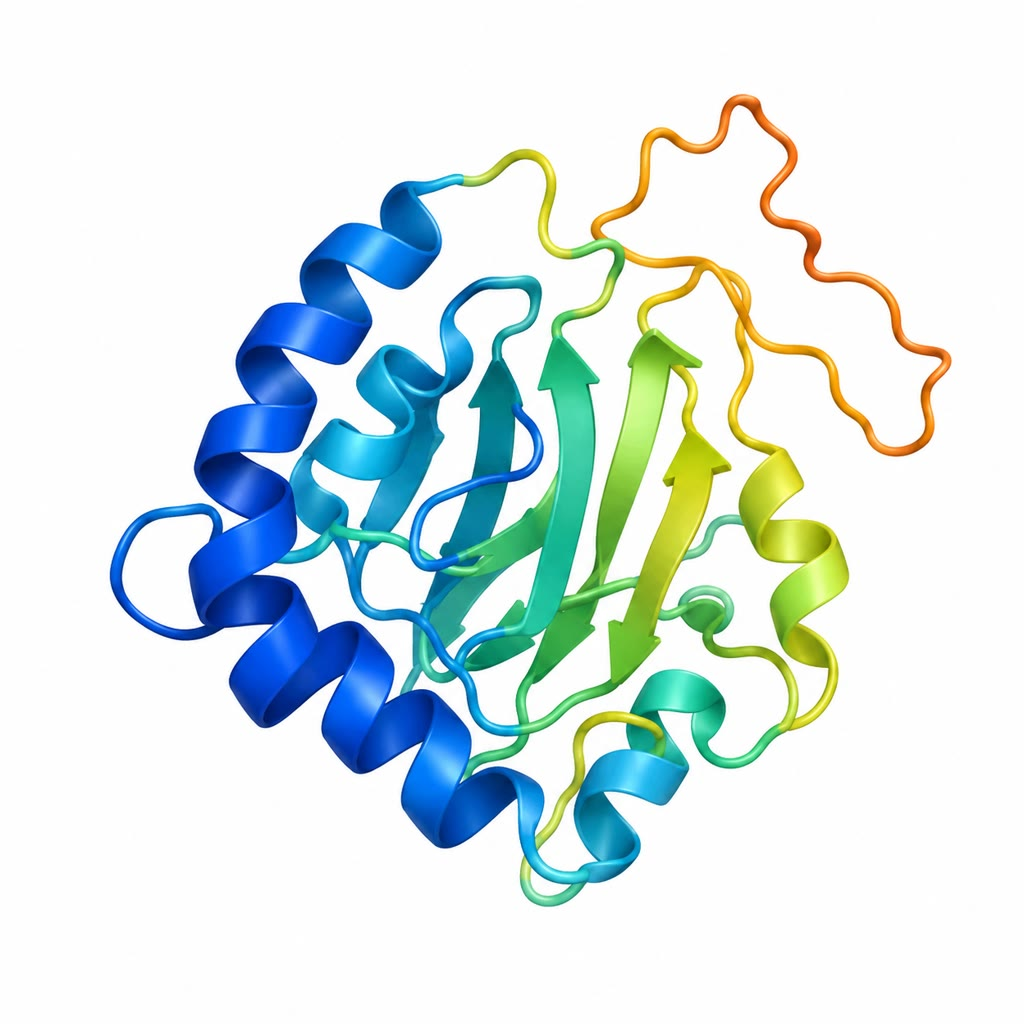
\includegraphics[width=0.36\linewidth]{images/book5/ai/b5-05-alphafold.jpg}\hspace{0.04\linewidth}
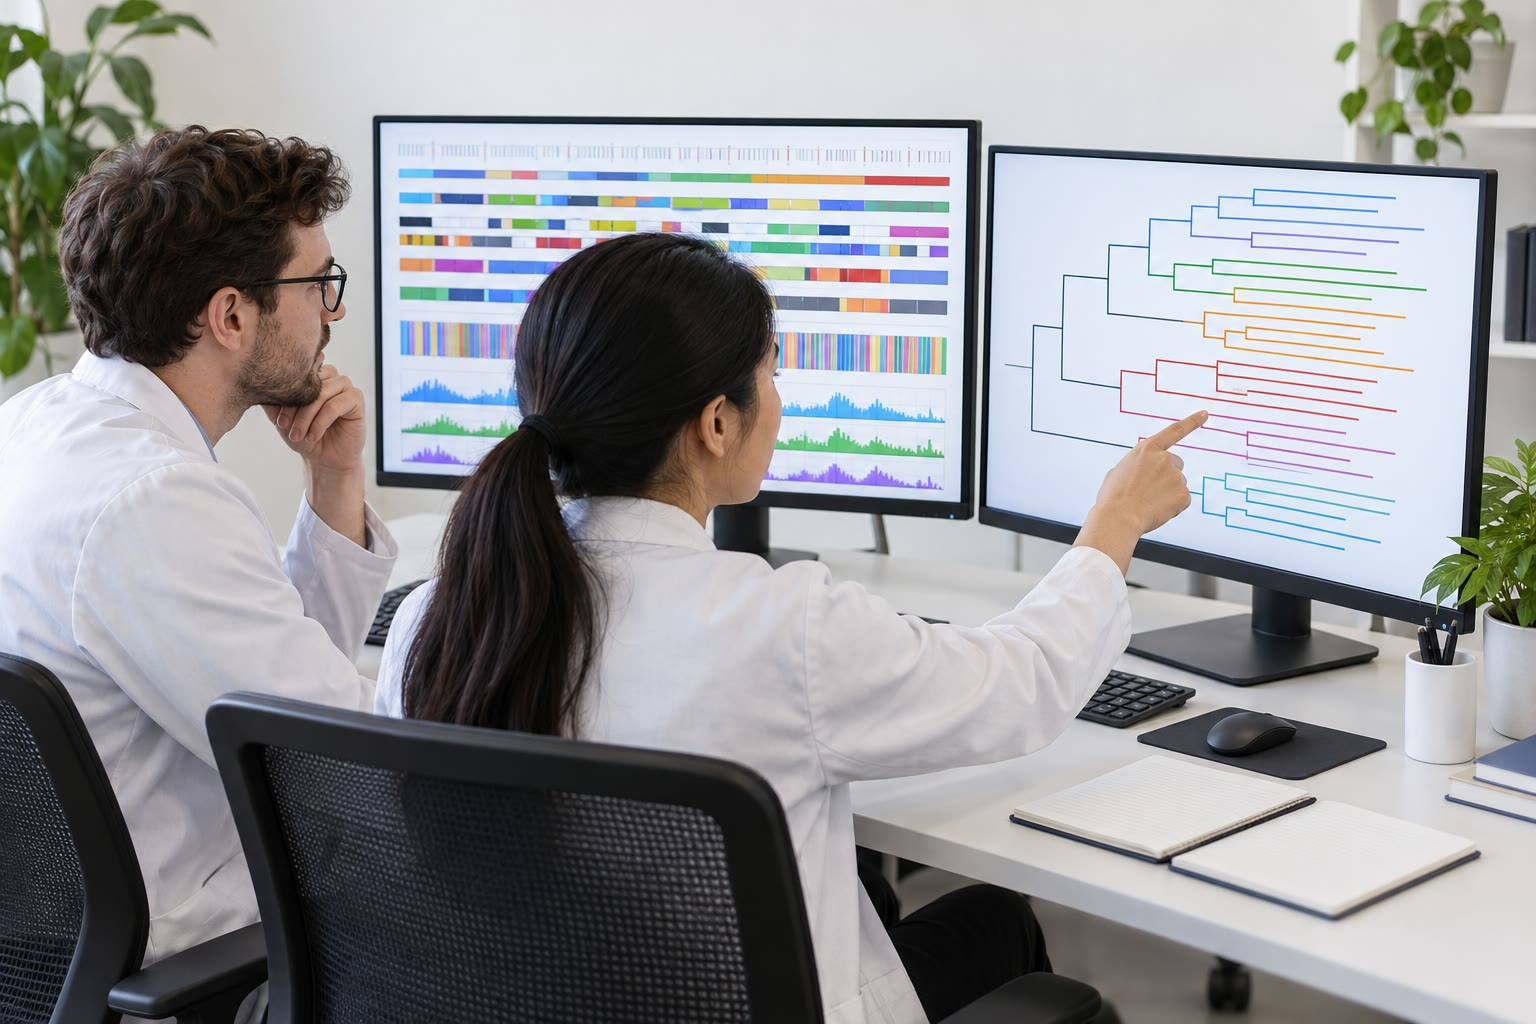
\includegraphics[width=0.54\linewidth]{images/book5/ai/b5-05-bioinformatics-lab.jpg}

{\small Izquierda: una estructura de proteína predicha, coloreada según
la confianza del modelo, de alta (azul) a baja (naranja) en un bucle
desordenado. Derecha: un despacho de bioinformática --- navegadores de
genomas y árboles en las pantallas, y ni un solo poyo de laboratorio a la
vista.}
\end{omfigure}

\begin{remark}[Los límites de la inferencia]\label{rem:b3:bioinformatics:limits}
La mayoría de las anotaciones funcionales de las bases de datos nunca se
pusieron a prueba; se transfirieron de un homólogo, que a su vez había
sido anotado por transferencia. Los errores se propagan y se multiplican,
y una \omterm{def:b3:genomics:assembly}{anotación} equivocada en una proteína bien conectada puede infectar
a toda una familia. Los remedios son los de más arriba: distíngase la
ortología de la homología, léase el \omterm{def:b3:bioinformatics:alignment}{alineamiento}, búsquense los residuos
catalíticos y recuérdese que ``proteína hipotética'' es una etiqueta
honrada que un tercio de los genes de la mayoría de los genomas todavía
merece.
\end{remark}

\section{Ejercicios}

\begin{exercise}[$\star$]\label{exo:b3:bioinformatics:1}
Defínanse el \omterm{def:b3:bioinformatics:alignment}{alineamiento global} y el local y dese una situación
biológica que reclame cada uno.
\end{exercise}

\begin{exercise}[$\star$]\label{exo:b3:bioinformatics:2}
Rellénese la tabla de Needleman--Wunsch de AGC contra AAC con
coincidencia $+1$, discrepancia $-1$ y hueco $-1$, y dense el
\omterm{def:b3:bioinformatics:alignment}{alineamiento} óptimo y su puntuación.
\end{exercise}

\begin{exercise}[$\star$]\label{exo:b3:bioinformatics:3}
En BLOSUM62, triptófano--triptófano puntúa $+11$ y leucina--leucina $+4$.
Explíquese a partir de la fórmula de log-verosimilitudes por qué la
identidad del residuo más raro vale más.
\end{exercise}

\begin{exercise}[$\star$]\label{exo:b3:bioinformatics:4}
¿Qué es un \omterm{thm:b3:bioinformatics:evalue}{valor E}? Una búsqueda devuelve un acierto con $E = 3$. ¿Qué
significa ese número, y es homólogo el acierto?
\end{exercise}

\begin{exercise}[$\star\star$]\label{exo:b3:bioinformatics:5}
Se busca una consulta de \num{400} residuos contra $2\times 10^{11}$
residuos. Calcúlense los \omterm{thm:b3:bioinformatics:evalue}{valores E} de los aciertos con puntuaciones en
bits $45$, $55$ y $65$. ¿Qué \omterm{thm:b3:bioinformatics:evalue}{puntuación en bits} da $E = 10^{-3}$? ¿Cómo
cambia la respuesta si la consulta mide \num{40} residuos?
\end{exercise}

\begin{exercise}[$\star\star$]\label{exo:b3:bioinformatics:6}
Calcúlese el \omterm{def:b3:bioinformatics:motif}{contenido de información} de un \omterm{def:b3:bioinformatics:motif}{motivo} cuyas cuatro
posiciones tienen frecuencias de bases (A, C, G, T) de $(1,0,0,0)$,
$(0.5,0,0.5,0)$, $(0.25,0.25,0.25,0.25)$ y $(0.7,0.1,0.1,0.1)$. ¿Cuántas
coincidencias por azar tiene en un genoma de \qty{4.6}{Mb}?
\end{exercise}

\begin{exercise}[$\star\star$]\label{exo:b3:bioinformatics:7}
Explíquese por qué las penalizaciones afines por hueco son más realistas
que las lineales, y por qué una penalización de apertura muy alta y una
muy baja dan las dos malos \omterm{def:b3:bioinformatics:alignment}{alineamientos}.
\end{exercise}

\begin{exercise}[$\star\star$]\label{exo:b3:bioinformatics:8}
Una búsqueda \omterm{def:b3:bioinformatics:blast}{BLAST} de una proteína humana contra una base de datos de
mosca da un mejor acierto con $E = 10^{-30}$ que cubre los residuos
50--180 de la consulta de \num{600} residuos. ¿Es la proteína de la mosca
el \omterm{def:b3:genomics:comparative}{ortólogo} de la humana? ¿Qué prueba adicional se haría?
\end{exercise}

\begin{exercise}[$\star\star$]\label{exo:b3:bioinformatics:9}
¿Por qué los métodos de \omterm{def:b3:bioinformatics:msa}{perfil} detectan homólogos que el \omterm{def:b3:bioinformatics:alignment}{alineamiento} por
pares pierde? Dese un ejemplo de patrón de columna que un \omterm{def:b3:bioinformatics:msa}{perfil} capta y
una secuencia aislada no.
\end{exercise}

\begin{exercise}[$\star\star\star$]\label{exo:b3:bioinformatics:10}
Muéstrese que, bajo un esquema de puntuación de esperanza positiva, el
\omterm{def:b3:bioinformatics:alignment}{alineamiento local} de Smith--Waterman de dos secuencias aleatorias largas
tiene una puntuación que crece linealmente con su longitud, y explíquese
por qué esto hace fracasar la teoría del \omterm{thm:b3:bioinformatics:evalue}{valor E}. ¿Qué implica para
alinear ADN con coincidencia $+1$ y discrepancia $-1$ a un \qty{60}{\%}
de contenido de GC?
\end{exercise}

\begin{exercise}[$\star\star\star$]\label{exo:b3:bioinformatics:11}
La tabla de Needleman--Wunsch necesita $mn$ celdas de memoria; para dos
cromosomas de \qty{100}{Mb} son $10^{16}$. Descríbanse dos ideas con las
que los alineadores de genomas lo evitan (\omterm{def:b3:bioinformatics:blast}{semillas} y encadenamiento;
bandas), y a qué renuncia cada una.
\end{exercise}

\begin{exercise}[$\star\star\star$]\label{exo:b3:bioinformatics:12}
Un modelo oculto de Markov de búsqueda de genes para bacterias tiene
estados para las tres posiciones del codón y para el ADN no codificante.
Explíquese cómo el modelo puede distinguir la secuencia codificante de la
no codificante sin información alguna sobre codones de parada
(considérese el uso de codones), y por qué el mismo enfoque es mucho más
difícil en un genoma humano.
\end{exercise}

\section{Problema: una secuencia del fondo del mar}

\begin{problem}[{Problema de fin de semana --- una proteína desconocida
alineada a mano, buscada en las bases de datos con su significación
calculada, su motivo regulador pesado en bits y su gen contrastado con la
estadística de los marcos de lectura abiertos aleatorios, hasta llegar al
valor E del mejor acierto, a los bits que necesita un sitio y a la
longitud que ha de tener un marco de lectura para creérselo}]
\label{pb:b3:bioinformatics:1}
Datos: una proteína de \num{300} residuos de un anélido abisal. Base de
datos de proteínas: $1.2\times 10^{11}$ residuos. Genoma del gusano:
\qty{1.6}{Gb}, \qty{38}{\%} de GC. Puntuación de los \omterm{def:b3:bioinformatics:alignment}{alineamientos} a
mano: coincidencia $+1$, discrepancia $-1$, hueco $-1$. \omterm{thm:b3:bioinformatics:evalue}{Puntuación en
bits} del mejor acierto \omterm{def:b3:bioinformatics:blast}{BLAST}: $92$; del décimo acierto: $38$.

\medskip
\noindent\textbf{Parte I --- A mano.}
\begin{enumerate}
  \item Alinéense los péptidos KQT y KAQT con la recurrencia de
        Needleman--Wunsch: escríbase la tabla y dense el \omterm{def:b3:bioinformatics:alignment}{alineamiento}
        óptimo y su puntuación.
  \item Repítase con Smith--Waterman (local) para GATCAT contra ACAT:
        hállense el mejor \omterm{def:b3:bioinformatics:alignment}{alineamiento local} y su puntuación.
  \item ¿Cuántas actualizaciones de celda cuesta un \omterm{def:b3:bioinformatics:alignment}{alineamiento global}
        de la proteína de \num{300} residuos contra una proteína de
        \num{450} residuos? ¿Y contra toda la base de datos?
  \item Si un ordenador ejecuta $10^{9}$ actualizaciones por segundo,
        ¿cuánto tarda el \omterm{def:b3:bioinformatics:alignment}{alineamiento} de la pregunta 3 contra toda la
        base de datos? ¿Por qué se usa \omterm{def:b3:bioinformatics:blast}{BLAST} en su lugar?
  \item Una puntuación de identidad de BLOSUM62 es $+4$ para la alanina
        ($p_{A} =
        0.074$) y $+11$ para el triptófano ($p_{W} = 0.013$). Con
        $\lambda = 0.347$ (unidades de medio bit), calcúlense la
        frecuencia objetivo $q_{AA}$ y $q_{WW}$ y la razón $q/p^{2}$ de
        cada una. Interprétese.
  \item Dos proteínas comparten el \qty{24}{\%} de identidad a lo largo
        de $250$ residuos. Dígase por qué la identidad por sí sola no
        puede zanjar aquí la homología y qué sí podría.
\end{enumerate}

\medskip
\noindent\textbf{Parte II --- La búsqueda.}
\begin{enumerate}[resume]
  \item Calcúlense $mn$ para la consulta contra la base de datos y
        $\log_{2}(mn)$.
  \item Calcúlense el \omterm{thm:b3:bioinformatics:evalue}{valor E} del mejor acierto ($S' = 92$) y el del
        décimo acierto ($S' = 38$).
  \item ¿Qué \omterm{thm:b3:bioinformatics:evalue}{puntuación en bits} corresponde a $E = 10^{-3}$ en esta
        búsqueda? ¿Y a $E = 1$?
  \item El mismo mejor acierto se encuentra cuando la base de datos ha
        crecido hasta $1.2\times 10^{12}$ residuos. ¿Su \omterm{thm:b3:bioinformatics:evalue}{valor E}?
  \item El décimo acierto alinea los residuos 200--260 de la consulta
        con un \qty{40}{\%} de identidad a lo largo de $60$ residuos.
        Usando el \omterm{thm:b3:bioinformatics:evalue}{valor E}, dígase si es prueba de homología y qué podría
        añadir una búsqueda por \omterm{def:b3:bioinformatics:msa}{perfil}.
  \item El mejor acierto es una quinasa humana, alineada a lo largo de
        los residuos 10--290. Su mejor acierto en el proteoma del gusano
        es la consulta. ¿Qué establece esta prueba recíproca, y qué no?
\end{enumerate}

\medskip
\noindent\textbf{Parte III --- Un \omterm{def:b3:bioinformatics:motif}{motivo}.}
\begin{enumerate}[resume]
  \item Aguas arriba del gen hay un sitio candidato de factor de
        transcripción de ocho posiciones con \omterm{def:b3:bioinformatics:motif}{contenidos de información}
        $2, 2, 1.6, 2, 0.8, 1.2, 0.4, 0.3$ bits. ¿$R$ total?
  \item ¿Cuántas coincidencias por azar tiene el \omterm{def:b3:bioinformatics:motif}{motivo} en el genoma de
        \qty{1.6}{Gb} (ambas hebras, $3.2\times 10^{9}$ posiciones)?
  \item El factor regula unos $200$ genes. ¿Cuántos bits necesitaría un
        \omterm{def:b3:bioinformatics:motif}{motivo} para especificar $200$ sitios por sí solo en este genoma?
  \item ¿Cuánto del déficit podría aportar un segundo \omterm{def:b3:bioinformatics:motif}{motivo} contiguo de
        $8$ bits, si los dos han de aparecer juntos con un espaciado
        fijo?
  \item Una posición con frecuencias $(0.5, 0.5, 0, 0)$ para (A, C, G,
        T): calcúlense su entropía y su \omterm{def:b3:bioinformatics:motif}{contenido de información}.
  \item Explíquese, con el argumento de la información, por qué los
        factores de transcripción bacterianos suelen tener sitios más
        largos y más conservados que los eucariotas.
\end{enumerate}

\medskip
\noindent\textbf{Parte IV --- El gen mismo.}
\begin{enumerate}[resume]
  \item En ADN aleatorio de composición de bases uniforme, ¿cuál es la
        probabilidad de que un codón sea de parada? ¿Cuál es el número
        esperado de codones antes de que aparezca una parada (una
        distribución geométrica)?
  \item El genoma del gusano tiene un \qty{38}{\%} de GC. Recalcúlense
        la probabilidad de que un codón al azar sea de parada (TAA, TAG,
        TGA) con las frecuencias de bases reales y la longitud esperada
        del marco de lectura. ¿En qué sentido empuja un contenido de GC
        bajo a la búsqueda de genes?
  \item ¿Cuál es la probabilidad de que un marco de lectura abierto al
        azar tenga al menos $100$ codones? ¿Y al menos $300$?
  \item En el genoma de \qty{1.6}{Gb}, seis marcos en dos hebras dan
        unos $3.2\times 10^{9}$ inicios de codón. ¿Cuántos marcos de
        lectura abiertos al azar de al menos $100$ codones se esperan?
        ¿Y de al menos $300$?
  \item Explíquese por qué ``marco de lectura abierto de más de $100$
        codones'' es un buscador de genes utilizable en una bacteria
        pero no en este genoma, y qué usa en su lugar un buscador de
        genes eucariota.
  \item El gen del gusano tiene seis exones de \qty{150}{bp} de media.
        Explíquese cómo las lecturas de secuenciación de ARN resuelven
        la estructura de exones que la secuencia genómica por sí sola
        deja ambigua.
  \item Resúmase: el \omterm{thm:b3:bioinformatics:evalue}{valor E} del mejor acierto (pregunta~8), los bits
        necesarios para especificar $200$ sitios (pregunta~15) y el
        número esperado de marcos de lectura al azar de $300$ codones en
        el genoma (pregunta~22).
\end{enumerate}
\end{problem}
